\section{Theorie} 
\label{sec:Theorie}
In diesem Kapitel werden die theoretischen Hintergründe dieses Versuches erläutert.


\subsection{Das Bändermodell}
\label{sec:baendermodell}
Ein einzelnes Atom besitzt nur diskrete Energiniveaus auf denen sich Elektronen befinden können. In einem 
Festkörper dürfen die Energieniveaus der Atome allerdings nicht vollständig gleich sein und unterscheiden sich 
daher minimal, sin aber dennoch nah genug beieinander das die Elektronen problemlos zwischen den Niveaus 
wechseln können, sie sind quasikontinuirlich. So ergeben sich die sogenannten Bänder. Bänder die vollständig 
mit Elektronen gefüllt sind tragen nicht zur elektrischen Leitfähigkeit bei, sie heißen Valenzbänder. 
Die Bänder sind im Energieraum ausgedehnt und können sich mit anderen Bändern überschneiden, oder durch eine 
Bandlücke voneinander getrennt sein. Bei einer großen Bandlücke und keinen Elektronen im Leitungsband
ist der Stoff ein Isolator. Hier ist die Bandlücke so groß das auch bei hohen Temperaturen keine nennenswerte Zahl
von Elektronen in das Leitungsband aufsteigen kann und so auch bei hohen Temperaturen keine elektrische
Leitfähigkeitentsteht. Bei einer schmalen Bandlücke ist der Stoff ein Halbleiter. Hier können durch thermische 
Anregung genug Elektronen ins Leitungsband aufsteigen um elektrische Leitfähigkeit zu gewährleisten. Am absoluten
Nullpunkt leiten intrinsische Halbleiter keinen Strom.
\begin{figure}
    \centering
    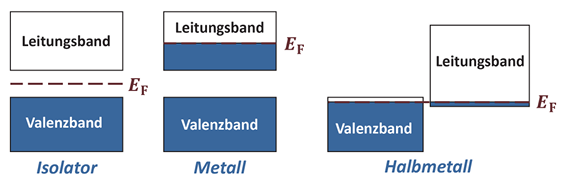
\includegraphics[width=1\textwidth]{content/grafiken/baender.JPG}
    \caption{Vergleich der Bändermodelle von Isolatoren, Leitern und Halbleitern. $E_F$ bezeichnet die Fermienergie [1]}
    \label{fig:baendermodell}
  \end{figure}


\subsection{Die effektive Masse}
\label{sec:effektiveMasse}
Elektronen können sich auch im Festkörper nicht als vollständig frei betrachtet werden. Sie spüren die 
ortsabhängigen Potentiale der Atomrümpfe. Daher wird die effektive Masse $m^{\star}$ eingeführt. 
Dank ihr können die Elektronen in Leitungs- und nicht vollständig besetztden Valenzbändern als freie Elektronen
mit der Dispersionsrelation
\begin{equation}
  \label{eq:dispersionsrelation}
  E(\vec{k})=E_0+\frac{\hbar^2k^2}{2m^{\star}}
\end{equation}
beschrieben werden. Dabei ist $m^{\star}$ durch 
\begin{equation*}
  m^{\star}=\hbar(\frac{\mathrm{d}^2E}{\mathrm{d}k_i\mathrm{d}k_j})^{-1}
\end{equation*}
gegeben.


\subsection{Dotierung}
\label{sec:dotierung}
Reine Halbleiter, die auch als intrinsisch bezeichnet werden, leiten zwar elektrischen Strom, allerdings nicht
besonders gut. Daher werden sie Dotiert. Das bedeutet es wird eine sehr geringe Zahl Fremdatome (etwa 1 
Fremdatom auf 10000 bis 100-millionen Halbleiteratome) in das Kristallgitter eingebracht. Jenachdem ob die 
eingebrachten Atome eine höhere oder geringere Wertigkeit als die Halbleiteratome haben spricht man von 
n- oder p-Dotierung.
\subsubsection{n-Dotierung}
\label{sec:ndotierung}
n-Dotierung bedeutet das in ein Kristallgitter aus vierwertigen Atomen, fünfwertige Fremdatome,
sogenannte Doatoren, eingebracht werden. Das fünfte Hüllenelektronen das nicht zur Kristallbindung
benötigt wird ist stark delokalisiert und damit quasi frei. So entstehen neue Energiniveaus knapp unterhalb
des Leitungsbandes und die Bandlücke wird schmaler. So wird die elektrische Leitfähigkeit drastisch erhöht, 
da thermisch angeregte Elektronen leichter ins Leitungsband wechseln können. Das zugehörige Bändermodell
ist in \autoref{fig:baendermodelldon} schematisch dargestellt.
\begin{figure}
  \centering
  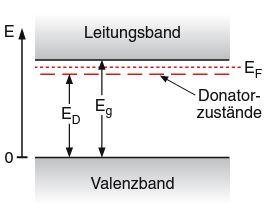
\includegraphics[width=1\textwidth]{content/grafiken/donatoren.JPG}
  \caption{Bändermodell eines mit donator Atomen dotierten Halbleiters. [3]}
  \label{fig:baendermodelldon}
\end{figure}
\subsubsection{p-Dotierung}
\label{sec:pdotierung}
p-Dotierung bedeutet das in das Kristallgitter aus vierwertigen Atomen die sogenannten Akzeptoren, also
dreiwertige Fremdatome eingebracht. Das führt dazu das dass Valenzband nach oben hin ausgeweitet wird.
Auch so wird die Bandlücke schmaler und die elektrische Leitfähigkeit wird stark erhöht. Das zugehörige 
Bändermodell ist in \autoref{fig:baendermodellakz} schematisch dargestellt.
\begin{figure}
  \centering
  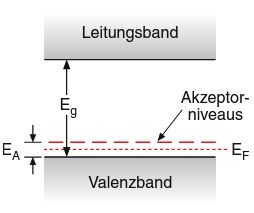
\includegraphics[width=1\textwidth]{content/grafiken/akzeptoren.JPG}
  \caption{Bändermodell eines mit akzeptor Atomen dotierten Halbleiters. [3]]}
  \label{fig:baendermodellakz}
\end{figure}


\subsection{Doppelbrechung}
\label{sec:doppelbrechung}
Ein zirkular polarisierter Lichtstrahl der in einen Kristall einläuft, der kein kubisches Kristallgitter 
besitzt, wird in zwei jeweils entgegengesetzt polarisierte teilsatrahlen aufgespalten. Die Begründung hierfür
liegt in Brechungsindizes die von der Polarisationsrichtung abhängen. Der eine, sogenannte ordentliche Strahl,
läuft ungebrochen durch den Kristall, der andere, sogenannte außerordentliche Strahl, wird vom ordentlichen
Strahl weggebrochen. Würde man den Kristall um die Strahlachse des ordentlichen Strahls rotieren würde der
außerordentliche Strahl sich auf einem Zylindermantel um den ordentlichen Strahl herum bewegen.
\subsubsection{Das Glan-Thompson-Prisma}
\autoref{sec:prisma}
Mithilfe der Doppelbrechung ist es möglich die im Versuch verwendeten Glan-Thompson-Prismen zu konstruieren.
Dafür wird ein doppelbrechender Kristall schräg in zwei Teile geschnitten und anschließend wieder zusammengefügt.
Der Schnittwinkel wird dabei so gewählt das der ordentliche Stahl an der Schnittebene totalreflektiert wird.
Das führt dazu das der Hauptstrahl nahezu verlustfrei in zwei senkrecht zueinander polarisierte Teilstrahlen 
aufgeteilt wird. Solche Prismen werden meist aus Kalkspat gefertigt da hier der Effekt der Doppelbrechung besonders
stark auftritt.
\subsection{Die zirkulare Doppelbrechung}
\label{sec:zdoppelbrechung}
Sogenannte optisch aktive Kristalle sorgen dafür das dass austretende linear polarisierte Licht zusätzlich noch 
eine veränderte polarisation besitzt. Das liegt an daran das in solchen Kristallen unterschiedliche Phasengeschwindigkeiten
abhängig von der Polarisationsrichtung existieren. Der einfallende linear polarisierte Lichtstrahl kann als Überlagerung von 
zwei in entgegengesetzte Richtungen zirkular polarisierte Wellen betrachtet werden. Die unterschiedlichen 
Phasengeschwindigkeiten führen dann bei späterer erneuter Überlagerung der beiden zirkular polarisierten Wellen wieder
zu dem resultierenden, linear polarisierten, jedoch gedrehtem Lichtstrahl.

\begin{figure}
  \centering
  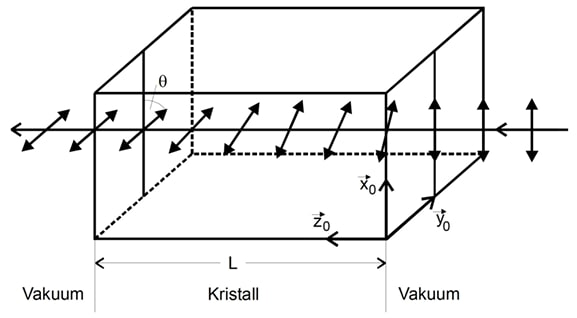
\includegraphics[width=1\textwidth]{content/grafiken/kristall.JPG}
  \caption{Drehung der Polarisationsebene einer elekromagnetischen Welle im B-Feld durchfluteten Medium. [1]}
  \label{fig:kristall}
\end{figure}

\subsection{Der Faradayeffekt}
\label{sec:faradayeffekt}
Ein isotroper lichtdurchlässiger Kristall der in ein entlang der Strahlachse gerichtetes Magnetfeld gebracht wird 
kann optisch aktiv werden. Das lässt sich damit begründen das das Magnetfeld zusätzliche Kreisströme in den Atomen 
des Kristalls bewirkt. So kommt es zu einer Asymetrie des Kristalls die sich durch das Magnetfeld quasi ein- und ausschalten
lässt. Der Drehwinkel $\theta$ der Polarisationsebene des durchlaufenden linear polarisierten Lichtstrahls ist abhängig
von dem durch die Verdet-Konstante $V$ repräsentierten Kristalls, der Länge $l$ des selbigen, sowie dss durchflutenden
Magnetfeldes $B$.
\begin{equation*}
  \theta=VBl
\end{equation*}
Die Besonderheit des Faradayeffektes gegenüber der normalen optischen Aktivität liegt darin das der Faradayeffekt von der 
Durchlaufrichtung des des Lichtstrahls abhängig ist. Wenn der Lichtstrahl also erst in die eine und dann in die andere Richtung 
durch das selbe Medium läuft ist die Polarisationsebene um den Winkel $2\theta$ gedreht. Bei normaler optischer Aktivität 
wäre bei einem solchen Aufbau am Ende keine Drehung mehr vorhanden.
\subsubsection{Berechnung des Rotationswinkels der Polarisationebene}
\label{sec:rotationsweinkel}
Die Bewegungsgleichung für ein gebundenes Elektron im Magnetfeld lautet:
\begin{equation*}
  m\frac{\mathrm{d}^2 \vec{r}}{\mathrm{d}t^2}+K\vec{r}=-e_0\vec{E}(\vec{r})\frac{\mathrm{d} \vec{r}}{\mathrm{d}t}\times \vec{B}.\\
\end{equation*}
Dabei ist $\vec{r}$ die Auslenkung des Elektrons aus seiner Ruhelage, $\vec{E}(\vec{r})$ das Feld der einfallenden Lichtwelle
und $\vec{B}$ das äußere Magnetfeld. Die Konstante $K$ beschreibt die Bindung des Elektrons an die Umgebung. Da das E-Feld eine
sehr hohe Kreisfrequenz $\omega$ aufweist kann nur eine Verschiebungspolarisation beobachtet werden und es gilt:
\begin{equation*}
  \vec{P}=-Ne_0 \vec{r}\\
\end{equation*} 

mit $N$ als Elektronendichte. Wenn nun ein Kristallsymetrie ernidrigendes Magnetfeld $\vec{B}$ angelegt treten im Suszeptibilitätstensor
$\chi$ nicht-diagonale Komponenten auf und es ergibt sich letztlich der Rotationswinkel $\theta$ zu:
\begin{equation*}
  \theta = \frac{e_0^3 \omega^2 NBl}{2\epsilon_0 cm^2((-\omega^2+\frac{K}{m})^2-(\frac{e_0B\omega}{m})^2)n}.\\
\end{equation*}
mit der elektrischen Feldkonstante $\epsilon_0$, der Lichtgeschwindigkeit $c$, der Probenlänge $l$, dem
Brechungsindex $n$, der Resonanzfrequenz $\omega_0:= \sqrt{\frac{K}{m}}$ der gebundenen Ladungsträger
und der Zyklotronfrequenz $\omega_c:=\epsilon_0\frac{B}{m}$ , welche die Umlauffrequenz der Ladungsträger
beschreibt, welche ohne weitere Einflüsse aufgrund der Lorentz-Kraft eine Kreisbahn um
die Feldachse $\vec{B}$ beschreiben würden. Für Messfrequenzen weit unter der Resonanzfrequenz
$\omega_0$ gilt die Näherung:
\begin{equation*}
  \theta \approx \frac{e_0^3 NBl}{2\epsilon_0cm^2\lambda^2\omega_0^4n}\\
\end{equation*}
wobei $\lambda$ die Wellenlänge des verwendeten Lichts repräsentiert. Für quasifreie Ladungsträger gilt aufgrund von $(\omega_0\rightarrow 0)$ im weiteren:
\begin{equation*}
  \theta \approx \frac{e_0^3\lambda^2NBl}{8\pi^2\epsilon_0c^3m^2n}.\\
\end{equation*}
In dieser Gleichung kann nun $m$ durch die effektive Masse $m^{\star}$ ersetzt werden, sodass jetzt  die quasifreien Elektronen in einem Kristall repräsentiert werden.
\begin{equation}
  \label{eq:thetafrei}
  \theta_{frei}=\frac{e_0^3\lambda^2NB}{8\pi^2\epsilon_0c^3(m^{\star})^2n}.\\
\end{equation}
wobei $\theta_{frei}=\frac{\theta}{L}$ die Faraday-Rotation pro Einheitslänge in $\frac{\mathrm{rad}}{\mathrm{m}}$ darstellt.